\documentclass{article}
\usepackage[margin=1in]{geometry}
\usepackage[linesnumbered,ruled,vlined]{algorithm2e}
\usepackage{amsfonts}
\usepackage{amsmath}
\usepackage{amssymb}
\usepackage{amsthm}
\usepackage{enumitem}
\usepackage{fancyhdr}
\usepackage{hyperref}
\usepackage{minted}
\usepackage{multicol}
\usepackage{pdfpages}
\usepackage{standalone}
\usepackage[many]{tcolorbox}
\usepackage{tikz-cd}
\usepackage{transparent}
\usepackage{xcolor}
% \tcbuselibrary{minted}

\author{Nathan Solomon}

\newcommand{\fig}[1]{
    \begin{center}
        \includegraphics[width=\textwidth]{#1}
    \end{center}
}

% Math commands
\renewcommand{\d}{\mathrm{d}}
\DeclareMathOperator{\id}{id}
\DeclareMathOperator{\im}{im}
\DeclareMathOperator{\proj}{proj}
\DeclareMathOperator{\Span}{span}
\DeclareMathOperator{\Tr}{Tr}
\DeclareMathOperator{\tr}{tr}
\DeclareMathOperator{\ad}{ad}
\DeclareMathOperator{\ord}{ord}
%%%%%%%%%%%%%%% \DeclareMathOperator{\sgn}{sgn}
\DeclareMathOperator{\Aut}{Aut}
\DeclareMathOperator{\Inn}{Inn}
\DeclareMathOperator{\Out}{Out}
\DeclareMathOperator{\stab}{stab}

\newcommand{\N}{\ensuremath{\mathbb{N}}}
\newcommand{\Z}{\ensuremath{\mathbb{Z}}}
\newcommand{\Q}{\ensuremath{\mathbb{Q}}}
\newcommand{\R}{\ensuremath{\mathbb{R}}}
\newcommand{\C}{\ensuremath{\mathbb{C}}}
\renewcommand{\H}{\ensuremath{\mathbb{H}}}
\newcommand{\F}{\ensuremath{\mathbb{F}}}

\newcommand{\E}{\ensuremath{\mathbb{E}}}
\renewcommand{\P}{\ensuremath{\mathbb{P}}}

\newcommand{\es}{\ensuremath{\varnothing}}
\newcommand{\inv}{\ensuremath{^{-1}}}
\newcommand{\eps}{\ensuremath{\varepsilon}}
\newcommand{\del}{\ensuremath{\partial}}
\renewcommand{\a}{\ensuremath{\alpha}}

\newcommand{\abs}[1]{\ensuremath{\left\lvert #1 \right\rvert}}
\newcommand{\norm}[1]{\ensuremath{\left\lVert #1\right\rVert}}
\newcommand{\mean}[1]{\ensuremath{\left\langle #1 \right\rangle}}
\newcommand{\floor}[1]{\ensuremath{\left\lfloor #1 \right\rfloor}}
\newcommand{\ceil}[1]{\ensuremath{\left\lceil #1 \right\rceil}}
\newcommand{\bra}[1]{\ensuremath{\left\langle #1 \right\rvert}}
\newcommand{\ket}[1]{\ensuremath{\left\lvert #1 \right\rangle}}
\newcommand{\braket}[2]{\ensuremath{\left.\left\langle #1\right\vert #2 \right\rangle}}

\newcommand{\catname}[1]{{\normalfont\textbf{#1}}}

\newcommand{\up}{\ensuremath{\uparrow}}
\newcommand{\down}{\ensuremath{\downarrow}}

% Custom environments
\newtheorem{thm}{Theorem}[section]

\definecolor{probBackgroundColor}{RGB}{250,240,240}
\definecolor{probAccentColor}{RGB}{140,40,0}
\newenvironment{prob}{
    \stepcounter{thm}
    \begin{tcolorbox}[
        boxrule=1pt,
        sharp corners,
        colback=probBackgroundColor,
        colframe=probAccentColor,
        borderline west={4pt}{0pt}{probAccentColor},
        breakable
    ]
    \color{probAccentColor}\textbf{Problem \thethm.} \color{black}
} {
    \end{tcolorbox}
}

\definecolor{exampleBackgroundColor}{RGB}{212,232,246}
\newenvironment{example}{
    \stepcounter{thm}
    \begin{tcolorbox}[
      boxrule=1pt,
      sharp corners,
      colback=exampleBackgroundColor,
      breakable
    ]
    \textbf{Example \thethm.}
} {
    \end{tcolorbox}
}

\definecolor{propBackgroundColor}{RGB}{255,245,220}
\definecolor{propAccentColor}{RGB}{150,100,0}
\newenvironment{prop}{
    \stepcounter{thm}
    \begin{tcolorbox}[
        boxrule=1pt,
        sharp corners,
        colback=propBackgroundColor,
        colframe=propAccentColor,
        breakable
    ]
    \color{propAccentColor}\textbf{Proposition \thethm. }\color{black}
} {
    \end{tcolorbox}
}

\definecolor{thmBackgroundColor}{RGB}{235,225,245}
\definecolor{thmAccentColor}{RGB}{50,0,100}
\renewenvironment{thm}{
    \stepcounter{thm}
    \begin{tcolorbox}[
        boxrule=1pt,
        sharp corners,
        colback=thmBackgroundColor,
        colframe=thmAccentColor,
        breakable
    ]
    \color{thmAccentColor}\textbf{Theorem \thethm. }\color{black}
} {
    \end{tcolorbox}
}

\definecolor{corBackgroundColor}{RGB}{240,250,250}
\definecolor{corAccentColor}{RGB}{50,100,100}
\newenvironment{cor}{
    \stepcounter{thm}
    \begin{tcolorbox}[
        enhanced,
        boxrule=0pt,
        frame hidden,
        sharp corners,
        colback=corBackgroundColor,
        borderline west={4pt}{0pt}{corAccentColor},
        breakable
    ]
    \color{corAccentColor}\textbf{Corollary \thethm. }\color{black}
} {
    \end{tcolorbox}
}

\definecolor{lemBackgroundColor}{RGB}{255,245,235}
\definecolor{lemAccentColor}{RGB}{250,125,0}
\newenvironment{lem}{
    \stepcounter{thm}
    \begin{tcolorbox}[
        enhanced,
        boxrule=0pt,
        frame hidden,
        sharp corners,
        colback=lemBackgroundColor,
        borderline west={4pt}{0pt}{lemAccentColor},
        breakable
    ]
    \color{lemAccentColor}\textbf{Lemma \thethm. }\color{black}
} {
    \end{tcolorbox}
}

\definecolor{proofBackgroundColor}{RGB}{255,255,255}
\definecolor{proofAccentColor}{RGB}{80,80,80}
\renewenvironment{proof}{
    \begin{tcolorbox}[
        enhanced,
        boxrule=1pt,
        sharp corners,
        colback=proofBackgroundColor,
        colframe=proofAccentColor,
        borderline west={4pt}{0pt}{proofAccentColor},
        breakable
    ]
    \color{proofAccentColor}\emph{\textbf{Proof. }}\color{black}
} {
    \qed \end{tcolorbox}
}

\definecolor{noteBackgroundColor}{RGB}{240,250,240}
\definecolor{noteAccentColor}{RGB}{30,130,30}
\newenvironment{note}{
    \begin{tcolorbox}[
        enhanced,
        boxrule=0pt,
        frame hidden,
        sharp corners,
        colback=noteBackgroundColor,
        borderline west={4pt}{0pt}{noteAccentColor},
        breakable
    ]
    \color{noteAccentColor}\textbf{Note. }\color{black}
} {
    \end{tcolorbox}
}


\fancyhf{}
\setlength{\headheight}{24pt}

\date{\today}
\title{Math 115B Homework \#7}

\begin{document}
\maketitle

\begin{prob}
\end{prob}
By theorem 6.24, an operator $T$ is an orthogonal projection iff $T^2=T=T^*$. So if $T$ is an orthogonal projection, then $T=T^*$.

\bigskip
\par
\begin{prob}
\end{prob}
\begin{enumerate}[label=(\alph*)]
    \item For any $v \in V$, $\norm{v}=\norm{T(v)}$. For any $w \in W$, $w$ is also in $V$, so $\norm{w}=\norm{T|_W(w)}$.
    \item Since $T|_W^*=T|_W^{-1}$, we know $T|_W$ is invertible, so it's a bijection from $W$ to $W$. That means $T^{-1}(w) \in W$ for any $w \in W$, so the preimage of $W$ under $T$. Conversely, $T$ cannot map any element of $W^\perp$ to a nonzero element of $W$, so $W^\perp$ is $T$-invariant.
    \item For any $v \in V$, $\norm{v}=\norm{T(v)}$. For any $w \in W^\perp$, $w$ is also in $V$, so $\norm{w}=\norm{T|_{W^\perp}(w)}$, meaning $T|_{W^\perp}$ is unitary.
\end{enumerate}


\bigskip
\par
\begin{prob}
\end{prob}
If $T$ is either a rotation or reflection on $V$, then there exists $\theta \in \R$ and a basis $\varepsilon = \{ e_1, e_2 \}$ of $V$ such that
\[ [T]_\varepsilon \in \left\{ \begin{bmatrix}
        1 & 0 \\
        0 & -1
\end{bmatrix}, \begin{bmatrix}
        \cos \theta & - \sin \theta \\
        \sin \theta & \cos \theta
\end{bmatrix} \right\}. \]
In the first case, $T$ is a reflection, and $T^*=T$. In the second case, $T$ is a rotation, and $T^*=T$. Either way, $T$ is unitary (which is equivalent to orthogonal, since $V$ is a real inner product space).
\par
The composition of any unitary operators $A, B$ is also unitary because for any $v \in V$,
\[ \norm{v}=\norm{Bv}=\norm{ABv}. \]

\bigskip
\par
\begin{prob}
\end{prob}
Define
\[ x_1 = \begin{bmatrix}
    \cos (\theta / 2) \\
    \sin (\theta / 2)
\end{bmatrix}, x_2 = \begin{bmatrix}
- \sin (\theta / 2) \\
\cos (\theta / 2)
\end{bmatrix}. \]
Then $Lx_1=x_1$ and $Lx_2=-x_2$. Therefore, $W=\Span(x_2)$ is a one-dimensional subspace such that $Lw=w$ for any $w \in W$ and $Lv=-v$ for any $v \in W^\perp$, meaning $L$ is a reflection about $W^\perp=\Span(x_1)$.


\bigskip
\par
\begin{prob}
\end{prob}
\begin{enumerate}[label=(\alph*)]
    \item Let $T$ be a rotation. Then $T$ is orthogonal, so $\norm{Te_1}=\norm{e_1}=1$. Therefore $Te_1$ is on the unit circle, so there exists $\theta \in \R$ such that
        \[ Te_1 = \begin{bmatrix}
            \cos \theta \\
            \sin \theta
        \end{bmatrix}. \]
        We also know $0=\mean{e_1, e_2}=\mean{Te_1, Te_2}$. Since $Te_2$ is perpendicular to $Te_1$, there exists a constant $a \in \R$ such that
        \[ Te_2 = \begin{bmatrix}
            -a \cdot \sin \theta \\
            a \cdot \cos \theta
        \end{bmatrix}. \]
        In matrix form, $T$ can be written as
        \[ [T]_\varepsilon = R_\theta = \begin{bmatrix}
            \cos \theta & - a \cdot \sin \theta \\
            \sin \theta & a \cdot \cos \theta
        \end{bmatrix}. \]
        The determinant of that is $a \cos^2 \theta - a (-\sin^2 \theta) = a$, but the determinant of an orthogonal matrix is always one, so $a=1$.
    \item \begin{align*}
            R_\theta R_\varphi &= \begin{bmatrix}
                \cos \theta & -\sin \theta \\
                \sin \theta & \cos \theta
            \end{bmatrix} \begin{bmatrix}
                \cos \varphi & -\sin \varphi \\
                \sin \varphi & \cos \varphi
            \end{bmatrix} \\
            &= \begin{bmatrix}
                \cos \theta \cos \varphi - \sin \theta \sin \varphi & -\cos \theta \sin \varphi - \sin \theta \cos \varphi \\
                \sin \theta \cos \varphi + \cos \theta \sin \varphi & \sin \theta \sin \varphi + \cos \theta \cos \varphi
            \end{bmatrix} \\
            &= \begin{bmatrix}
                \cos(\theta + \varphi) & -\sin(\theta + \varphi) \\
                \sin(\theta + \varphi) & \cos(\theta+\varphi)
            \end{bmatrix} \\
            &= R_{\theta + \varphi}.
    \end{align*}
    \item
        \[ R_\theta R_\varphi = R_{\theta+\varphi}=R_{\varphi+\theta}=R_\varphi R_\theta. \]
\end{enumerate}

\bigskip
\par
\begin{prob}
\end{prob}
From the previous few problems, it is obvious that the determinant of a rotation is one.
\par
If $T$ is a reflection, then there exists a one dimensional subspace $W$ such that $Tx=-x$ for any $x \in W$ and $Tx=x$ for any $x \in W^\perp$. Therefore $T$ is diagonaizable, one of its eigenvalues is $-1$, and the rest are $1$. That means $\det{T}=-1$, so $T$ cannot also be a rotation.

\bigskip
\par
\begin{prob}
\end{prob}
$T$ is a direct sum of rotations iff it can be written as the composition of rotation operators. If $\dim(V)$ is odd, then $\det(T)=\det(-I_V)=(-1)^{\dim(V)}=-1$. Rotation operators always have determinant one, so their composition also does, so $T$ cannot be a direct sum of rotations.
\par
If $\dim(V)$ is even, then let $v_1, v_2, \dots, v_{2n}$ be an orthonormal basis of $V$, let $W_i =\Span \left\{ v_{2i-1}, v_{2i} \right\}$, and let $R_i$ be the rotation of $W_i$ by $\pi$ radians. Then $T=R_1 \oplus R_2 \oplus \cdots \oplus R_n$.
\par

\bigskip
\par
\begin{prob}
\end{prob}
Since $v$ and $w$ both lie on the unit circle, there exists $\theta, \varphi \in \R$ such that
\[ v = \begin{bmatrix}
    \cos \theta \\
    \sin \theta
\end{bmatrix}, w = \begin{bmatrix}
    \cos \varphi \\
    \sin \varphi
\end{bmatrix}. \]
Then $R_\theta e_1=v$ and $R_\varphi e_1 = w$, so
\begin{align*}
    R_{\varphi-\theta} v &= R_\varphi R_{-\theta} v \\
                         &= R_\varphi R_\theta^{-1} v \\
                         &= R_\varphi e_1 \\
                         &= w.
\end{align*}
Suppose there is another rotation, $R_\phi$, such that $R_\phi v = w$. Then $v = R_\phi^{-1} w = R_\phi^{-1} R_{\varphi-\theta} v = R_{\varphi-\theta-\phi} v$. The only 2D rotation which maps a nonzero vector $v$ to itself is the identity, $R_0$, so $\varphi-\theta-\phi \in 2\pi \Z$. That would mean $R_\phi=R_{\varphi-\theta}$, so the rotation is unique.

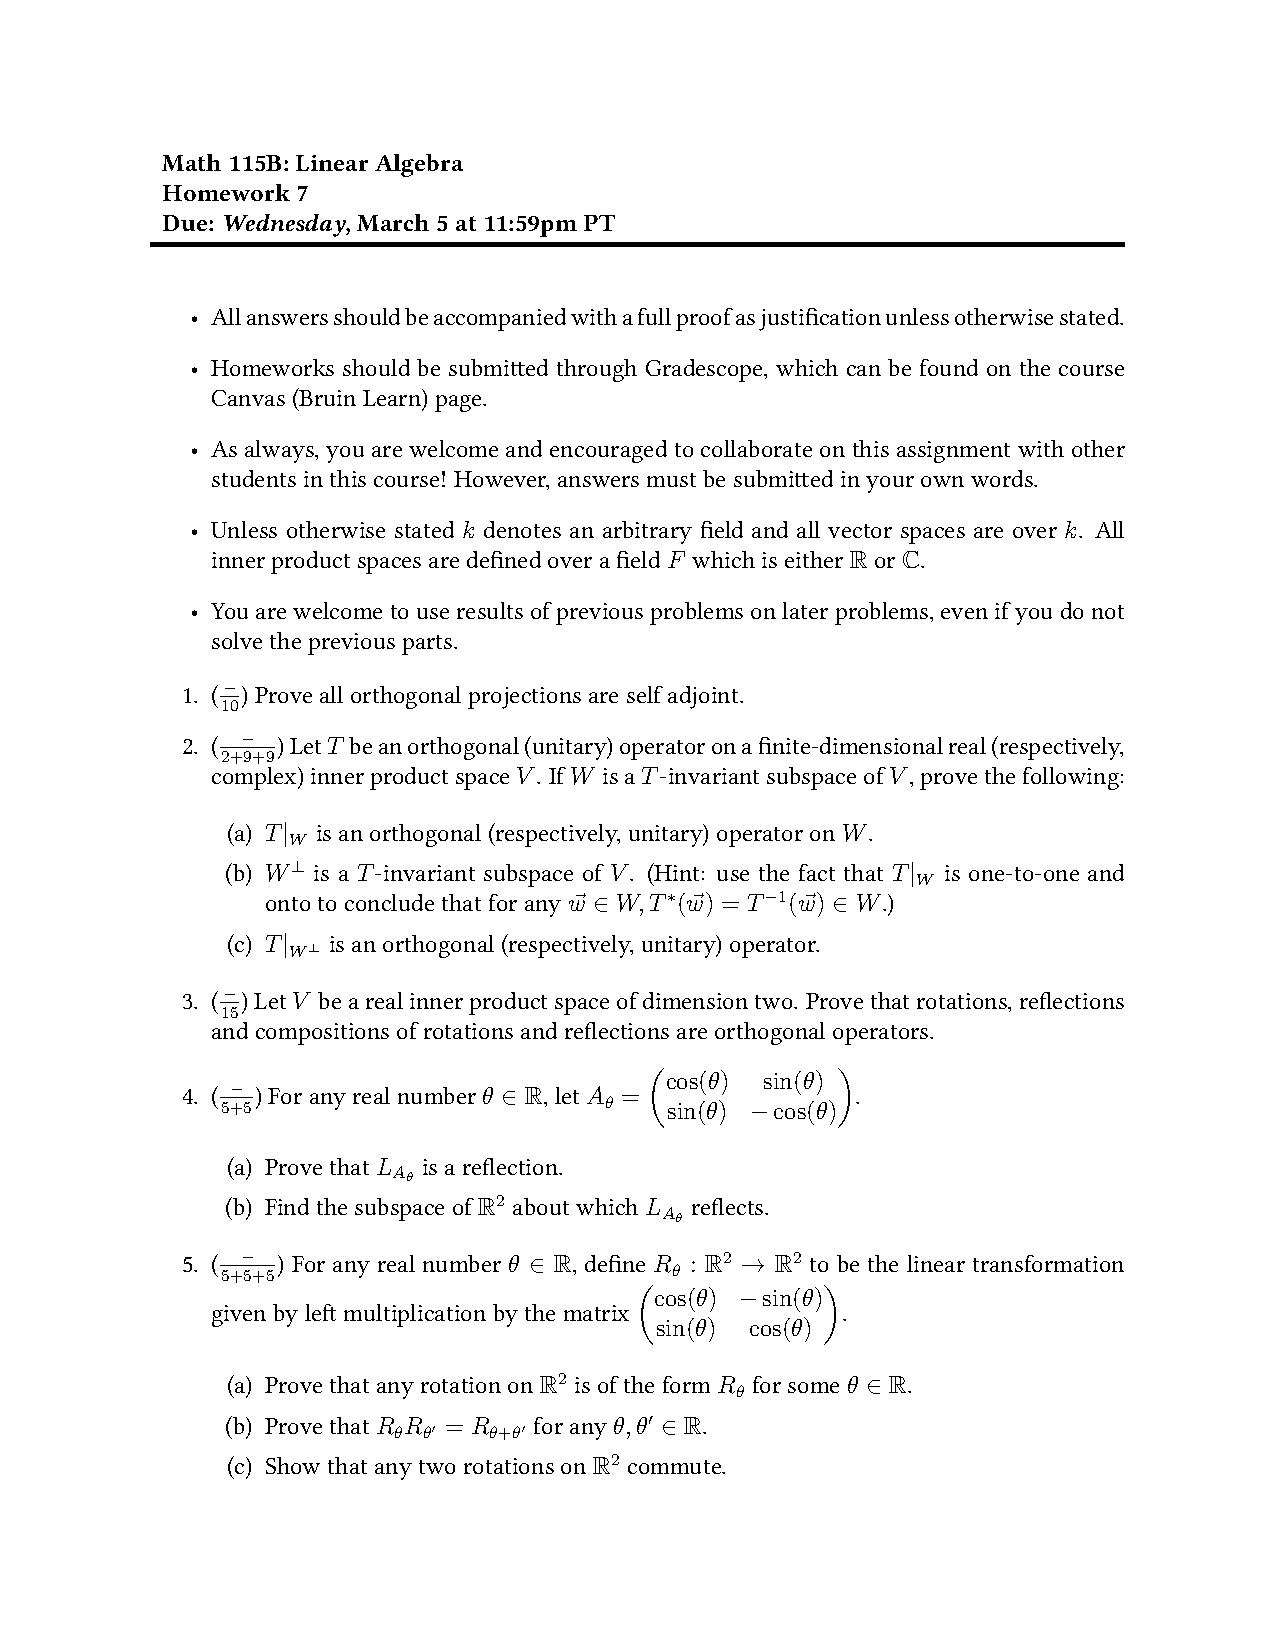
\includepdf[pages=-]{assignment.pdf}

\end{document}
